\documentclass[compress]{beamer}
\useoutertheme{miniframes}
\useinnertheme{rectangles}
\usecolortheme{orchid}
\usepackage{pgfpages,graphicx,epstopdf, bm,ifthen}
\usepackage[english]{babel}
\usepackage[T1]{fontenc}
\usepackage{latexsym,times,graphics,fancybox,fancyhdr,bm, amssymb,amsmath,amsthm}
\usepackage[english]{babel}
\usepackage{multicol,fancyvrb,color}
\usepackage{animate}

\defbeamertemplate{headline}{my header}{%
	\vskip1pt%
	\insertshorttitle%
}

\setbeamertemplate{headline}[my header]
\defbeamertemplate{footline}{my footer}{%
	\vskip1pt%
	\setbeamertemplate{footline}[page number]%
	\usebeamertemplate{footline}%
}

\setbeamertemplate{footline}[my footer]
\setbeamertemplate{navigation symbols}{} %gets rid of navigation symbols
\newcommand{\heading}[1]{\begin{center}\huge\bf\shadowbox{#1}\end{center}
	\vspace{1ex minus 1ex}}

\AtBeginSection[]{\begin{frame}\frametitle{Outline}
	\tableofcontents[currentsection,currentsubsection]\end{frame}}
\definecolor{darkred}{rgb}{0.62,0.18,0.18}
\newcommand{\change}[1]{\textcolor{darkred}{#1}}

\usefonttheme[stillsansseriftext]{serif}

\title['26 MA 551]{ Adam: Adaptive Moment Estimation}
\author{}
\date{}

\begin{document}

%------------------------------------------------
\begin{frame}
\titlepage
\end{frame}

%------------------------------------------------
\begin{frame}{Optimization problem}
We want to minimize (or maximize) an objective
\[
\min_{\theta \in \mathbb{R}^d} f(\theta),
\]
typically of the form
\[
f(\theta) = \mathbb{E}_{\xi}[\,\ell(\theta;\xi)\,]
\quad \text{or} \quad
\frac{1}{n}\sum_{i=1}^n \ell(\theta;i).
\]

Common in:
\begin{itemize}
\item Machine learning and deep learning
\item Large-scale stochastic optimization
\item Nonconvex problems
\end{itemize}
\end{frame}

%------------------------------------------------
\begin{frame}{From gradient descent to stochastic gradients}
Deterministic gradient descent:
\[
\theta_{t+1} = \theta_t - \eta_t \nabla f(\theta_t).
\]

Stochastic gradient descent (SGD):
\[
\theta_{t+1} = \theta_t - \eta_t g_t,
\qquad
\mathbb{E}[g_t \mid \theta_t] = \nabla f(\theta_t).
\]

Issues with SGD:
\begin{itemize}
\item Noisy gradients
\item Sensitive to learning-rate choice
\item Same step size for all coordinates
\end{itemize}
\end{frame}

%------------------------------------------------
\begin{frame}{Motivation for Adam}
Adam addresses two key issues in SGD:
\begin{itemize}
\item \textbf{Noise}: smooth gradients using momentum
\item \textbf{Scaling}: adapt step sizes per coordinate
\end{itemize}

Core ideas:
\begin{itemize}
\item Track first moment (mean) of gradients
\item Track second moment (variance) of gradients
\item Normalize updates using both
\end{itemize}
\end{frame}

%------------------------------------------------
\begin{frame}{Adam as a statistical estimator}
Reframe: Adam is a \textbf{method of moments estimator} applied online.

\medskip
At each step $t$, Adam maintains running estimates of the gradient distribution:
\[
m_t \approx \mathbb{E}[g_t], \qquad v_t \approx \mathbb{E}[g_t \odot g_t].
\]

The update is a \textbf{normalized score direction}:
\[
\theta_{t+1} = \theta_t - \eta \cdot \frac{\hat{m}_t}{\sqrt{\hat{v}_t} + \epsilon}
\approx \theta_t - \eta \cdot \frac{\mathbb{E}[g]}{\sqrt{\mathbb{E}[g^2]}}.
\]

\medskip
\textbf{Key insight:} The denominator $\sqrt{\hat{v}_t}$ approximates the \emph{standard deviation} of past gradients per coordinate --- a form of \textbf{online whitening}.

\medskip
This is why Adam is robust: it standardizes the gradient signal coordinate-wise at every step.
\end{frame}

%------------------------------------------------
\begin{frame}{First and second moments}
Given stochastic gradient $g_t$:

\textbf{First moment (momentum):}
\[
m_t = \beta_1 m_{t-1} + (1-\beta_1) g_t
\]

\textbf{Second moment (RMS scaling):}
\[
v_t = \beta_2 v_{t-1} + (1-\beta_2) g_t \odot g_t
\]

where:
\begin{itemize}
\item $\beta_1 \in [0,1)$ controls momentum
\item $\beta_2 \in [0,1)$ controls variance smoothing
\item $\odot$ denotes elementwise square
\end{itemize}
\end{frame}

%------------------------------------------------
\begin{frame}{Bias correction}
Since $m_0=v_0=0$, early estimates are biased toward zero.

Bias-corrected moments:
\[
\hat m_t = \frac{m_t}{1-\beta_1^t},
\qquad
\hat v_t = \frac{v_t}{1-\beta_2^t}.
\]

This correction is important in early iterations when $t$ is small.
\end{frame}

%------------------------------------------------
\begin{frame}{Adam update rule}
Adam parameter update:
\[
\boxed{
\theta_{t+1}
=
\theta_t
-
\eta
\frac{\hat m_t}{\sqrt{\hat v_t}+\epsilon}
}
\]

Components:
\begin{itemize}
\item numerator: smoothed gradient direction
\item denominator: coordinate-wise scaling
\item $\epsilon > 0$: numerical stability
\end{itemize}
\end{frame}

%------------------------------------------------
\begin{frame}{Adam algorithm (plain pseudocode)}
\textbf{Input:} step size $\eta$, parameters $\beta_1,\beta_2,\epsilon$

\medskip
\textbf{Initialize:} $\theta_1$, $m_0=0$, $v_0=0$, $t=0$

\medskip
\textbf{Repeat}:
\begin{itemize}
\item $t \leftarrow t+1$
\item Sample mini-batch and compute stochastic gradient $g_t$
\item Update moments:
\[
m_t=\beta_1 m_{t-1}+(1-\beta_1)g_t,
\quad
v_t=\beta_2 v_{t-1}+(1-\beta_2)g_t\odot g_t
\]
\item Bias correction:
\[
\hat m_t=\frac{m_t}{1-\beta_1^t},
\quad
\hat v_t=\frac{v_t}{1-\beta_2^t}
\]
\item Update parameters:
\[
\theta_{t+1}=\theta_t-\eta\frac{\hat m_t}{\sqrt{\hat v_t}+\epsilon}
\]
\end{itemize}

\medskip
\textbf{Output:} final or averaged iterate
\end{frame}

%------------------------------------------------
\begin{frame}{Interpretation of Adam}
Adam combines:
\begin{itemize}
\item \textbf{Momentum} (like heavy-ball / Polyak)
\item \textbf{Adaptive scaling} (like AdaGrad / RMSProp)
\end{itemize}

Effects:
\begin{itemize}
\item Large gradients $\Rightarrow$ smaller effective steps
\item Small gradients $\Rightarrow$ larger effective steps
\item Reduced sensitivity to learning-rate tuning
\end{itemize}

\medskip
\begin{center}
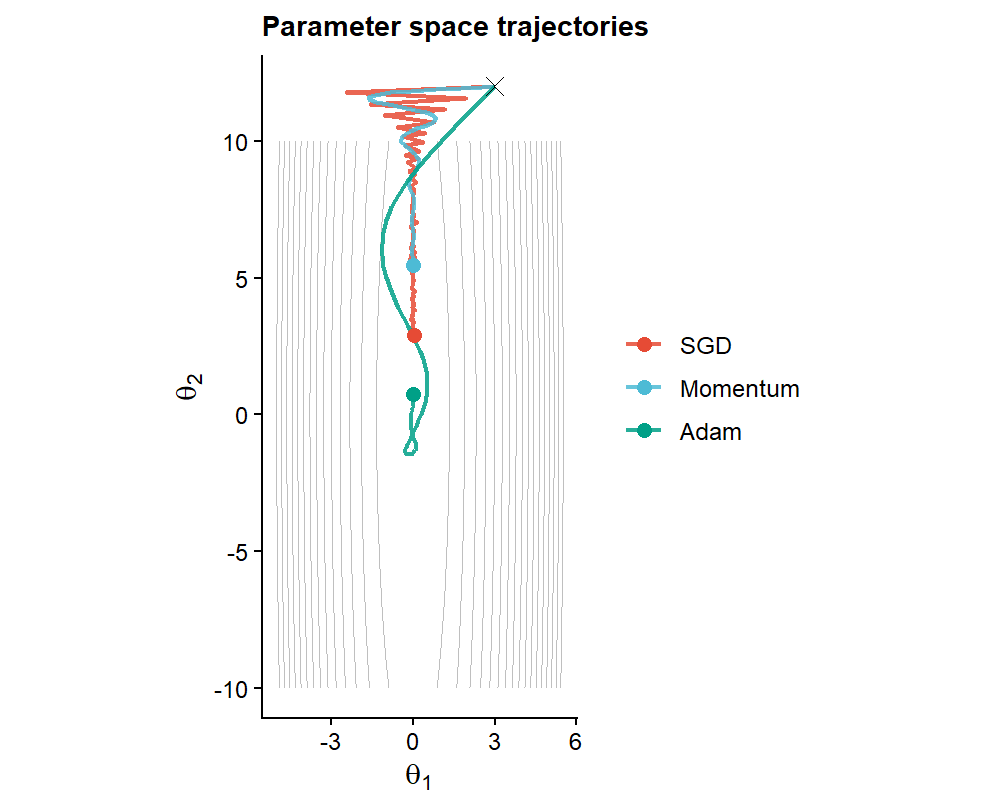
\includegraphics[width=0.72\linewidth]{optimizer_trajectories.png}

{\small Trajectories on anisotropic quadratic: SGD oscillates, Momentum overshoots, Adam navigates efficiently.}
\end{center}
\end{frame}

%------------------------------------------------
\begin{frame}{Comparison: SGD, Momentum, Adam}
\begin{center}
\animategraphics[loop, autoplay, width=\linewidth]{10}{gif_frames/frame}{000}{080}
\end{center}
{\small Left: parameter-space trajectories. Right: loss vs.\ iteration.}
\end{frame}

%------------------------------------------------
\begin{frame}{Typical hyperparameters}
Common default values:
\[
\beta_1 = 0.9,
\qquad
\beta_2 = 0.999,
\qquad
\epsilon = 10^{-8}.
\]

Learning rate:
\[
\eta \in [10^{-4}, 10^{-2}] \quad \text{(problem dependent)}.
\]

Defaults work surprisingly well, but tuning can still matter.
\end{frame}

%------------------------------------------------
\begin{frame}{Convergence considerations}
Adam performs well empirically, but theory is subtle.

Key points:
\begin{itemize}
\item Original Adam may fail to converge in some convex settings
\item Modified variants (e.g.\ AMSGrad) restore convergence guarantees
\item In practice, Adam converges reliably for many nonconvex problems
\end{itemize}

Theory typically shows convergence to stationary points under assumptions.
\end{frame}

%------------------------------------------------
\begin{frame}{Practical tips}
\begin{itemize}
\item Combine Adam with learning-rate decay or warmup
\item Use gradient clipping for stability
\item Monitor effective step size $\|\eta \hat m_t/\sqrt{\hat v_t}\|$
\item For final convergence, sometimes switch to SGD
\end{itemize}
Adam is excellent for fast progress, not always for final precision.
\end{frame}

%------------------------------------------------
\begin{frame}{Common pitfalls}
\begin{itemize}
\item Too large $\eta$ $\Rightarrow$ instability despite adaptivity
\item Poor generalization in some settings compared to SGD
\item Over-reliance on defaults without diagnostics
\item Ignoring convergence criteria (gradient norms)
\end{itemize}
Adam is powerful, but not magic.
\end{frame}

%------------------------------------------------
\begin{frame}{Connection to weak lensing}
Adam is the optimizer in \textbf{ShearNet}, a neural network for weak gravitational lensing shear estimation.

\medskip
Why Adam fits naturally:
\begin{itemize}
\item Noisy gradients: galaxy images are shot-noise limited
\item Anisotropic loss landscape: shear components $(\gamma_1, \gamma_2)$ and PSF parameters operate on different scales
\item Coordinate-wise adaptivity handles the heterogeneous parameter space automatically
\end{itemize}

\medskip
The statistical framing is literal here: $m_t$ and $v_t$ track the empirical gradient distribution over a stochastic mini-batch of simulated galaxy observations.

\medskip
{\small This is a direct application of online moment estimation to an astronomical inverse problem.}
\end{frame}

%------------------------------------------------
\begin{frame}{Takeaways}
\begin{itemize}
\item Adam adapts step sizes using first and second moments of gradients
\item Combines momentum and RMS normalization
\item Highly effective for large-scale, noisy, nonconvex optimization
\item Default optimizer in many modern ML systems
\end{itemize}

\[
\boxed{
\text{Adam: adaptive, robust, scalable stochastic optimization}
}
\]
\end{frame}

\end{document}